\chapter{Discrete-Time Stochastic Optimal Control}
\label{ch:discrete_time_stochastic_optimal_control}

\section{Sequential Decision Problems}
In sequential decision problems, an agent interacts with an environment by
selecting a series of actions in order to complete a specific task. During this
interaction, the agent receives a numerical reward from the environment and his
goal is to find the best strategy in order to maximize a certain measure of his
performance. The environment evolves stochastically and may be influenced by
the interaction with the agent, so that each action taken by the agent may 
influence the circumstances under which future decisions will be made. 
Therefore, the agent must balance his desire to obtain a large reward today 
by acting greedily and the opportunities that will be available in the future. 
While this setting appears quite simple, it is general enough to encompasses a 
wide range of applications in different fields. A classical example is 
portfolio management, where an investor must allocate his capital so as to 
maximize his long-term profits. Another standard example is chess, where two
players successively move pieces around the chessboard to checkmate the
opponent's king.\\
The purpose of the following sections is to introduce the notation that will be
used in the rest of this work and to recall the fundamental concepts and 
results of the discrete-time stochastic optimal control theory, which is the 
standard framework to study sequential decisions problems in mathematical
terms. Since our discussion will be far from being comprehensive, we refer the
reader to the extensive literature on the subject, such as
\cite{bertsekas1978stochastic}, \cite{puterman1994markov}, 
\cite{bertsekas1995dynamic}.

\section{Markov Decision Processes}
A sequential decision problem under uncertainty can be schematized as in Figure
\ref{fig:sequential_decision_problem}: at a given time $t$, the agent (also
known as decision maker or controller) observes the state $s_t$ of the system 
(also know as environment) and subsequently performs an action $a_t$. Following
this action, the agent receives an immediate reward $r_{t+1}$ (or incurs an
immediate cost) and the system evolves to a new state according to a probability
distribution which depends on the action selected by the agent. At the
subsequent time $t+1$, the agent selects a new action given the new state of
the system and the process repeats. This interaction can be modeled rigorously
using Markov decision processes.  
\begin{definition}[Markov Decision Process]
	A Markov decision process (MDP) is a stochastic dynamical system specified by the tuple $<\S, \A, \calP, \calR,
	\gamma>$, where
	\begin{enumerate}[label={\roman*)}]
		\item $(\S, \calS)$ is a measurable space, called the state space.
		\item $(\A, \calA)$ is a meausrable space, called the action space. 
		\item $\calP: \S \times \A \times \calS \to \R$ is a Markov transition
			kernel, i.e.
			\begin{enumerate}[label={\alph*)}]
				\item for every $s\in\S$ and $a\in\A$, $B \mapsto \calP(s,a,B)$
					  is a probability distribution over $(\S, \calS)$.
				\item for every $B\in\calS$, $(s,a) \mapsto \calP(s,a,B)$ is
					  a measurable function on $\S \times \A$.
			\end{enumerate}
		\item $\calR: \S \times \A \to \R$ is a reward function.
		\item $\gamma \in (0,1)$ is a discount factor.
	\end{enumerate}
\end{definition}
Typically, the state space (and similarly the action space) will be either
finite, i.e. $\S = \{s_1, \ldots, s_d\}$, or continuous, i.e. $\S \subseteq
\R^{D_s}$. The kernel $\calP$ describes the random evolution of the system:
suppose that at time $t$ the system is in state $s$ and that the agent takes
action $a$, then, regardless of the previous history of the system, the
probability to find the system in a state belonging to $B\in\calS$ at time
$t+1$ is given by $\calP(s, a, B)$, i.e.  \begin{equation}
	\calP(s, a, B) = \P{S_{t+1} \in B | S_t = s, A_t = a}
\end{equation}
Following this random transition, the agent receives a stochastic reward
$R_{t+1}$. The reward function $\calR(s, a)$ gives the expected reward
obtained when action $a$ is taken in state $s$, i.e. 
\begin{equation}
	\calR(s, a) = \E{R_{t+1} | S_t = s, A_t = a}
\end{equation}
This setting can be easily generalized to the following cases
\begin{enumerate}
	\item The initial state of the system is a random variable $S_0 \sim \mu$. 
	\item The actions that an agent can select depend on the state of the system.
\end{enumerate}

\begin{figure}[htpb]
	\centering
	\begin{tikzpicture}[node distance = 6em, auto, thick]
		\node [block] (Agent) {Agent};
		\node [block, below of=Agent] (Environment) {Environment};		    
		\path [line] (Agent.0) --++ (4em,0em) |- node [near start]{Action $a_t$} (Environment.0);
		\path [line] (Environment.190) --++ (-6em,0em) |- node [near start]{State  $s_{t}$} (Agent.170);
		\path [line] (Environment.170) --++ (-4.25em,0em) |- node [near start, right] {Reward $r_{t+1}$} (Agent.190);
	\end{tikzpicture}
	\caption{Agent-environment interaction in sequential decision problems.}
	\label{fig:sequential_decision_problem}
\end{figure}

\section{Policies}
At any time step, the agent selects his actions according to a certain policy. 
\begin{definition}[Policy]
	A policy is a function $\pi: \S \times \calA \to \R$ such that
	\begin{enumerate}[label={\roman*)}]
		\item for every $s \in \S$, $C \mapsto \pi(s,C)$ is a probability
			  distribution over $(\A, \calA)$. 
		\item for every $C \in \calA$, $s \mapsto \pi(s, C)$ is a measurable
			  function. 
	\end{enumerate}
\end{definition}
Intuitively, a policy represents a stochastic mapping from the current state of
the system to actions. Deterministic policies are a particular case of this 
general definition. We assumed that the agent's policy is stationary and only
depends on the current state of the system. We might in fact  consider more 
general policies that depends on the whole history of the system. However, as
we will see, we can always find an optimal policy that depends only on the
current state, so that our definition is not restrictive. A policy $\pi$ and an
initial state $s_0 \in \S$ determine a random state-action-reward sequence
${\{(S_t, A_t, R_{t+1})\}}_{t\geq 0}$ with values on $\S \times \A \times \R$
following the mechanism described above. 
\begin{definition}[History]
	Given an initial state $s_0 \in \S$ and a policy $\pi$, a history (or
	equivalently trajectory or roll-out) of the system is a random sequence
	$H_\pi = {\{(S_t, A_t)\}}_{t\geq 0}$ with values in $\S \times \A$, defined
	on some probability space $(\Omega, \mathcal{F}, \mathbb{P})$, such that for 
	$t = 0, 1, \ldots$
	\begin{equation*}
		\begin{cases}
			S_0 = s_0\\
			A_t \sim \pi(S_t, \cdot)\\
			S_{t+1} \sim \calP(S_t, A_t, \cdot)\\
		\end{cases}
	\end{equation*}
	we will denote by $(\H, \calH)$ the measurable space of all possible
	histories. 
\end{definition}
Moreover, we observe that
\begin{enumerate}[label={\roman*)}]
	\item the state sequence ${\{S_t\}}_{t\geq 0}$ is a Markov process $<\S,
		  \calP_\pi>$
	  \item the state-reward sequence ${\{(S_t, R_t)\}}_{t\geq 0}$ is a Markov 
		  reward process $<\S, \calP_\pi, \calR_\pi, \gamma>$
\end{enumerate}
where we denoted 
\begin{equation*}
	\begin{split}
		\calP_\pi(s, s') &= \int_\A \pi(s, a) \calP(s, a, s') da\\
		\calR_\pi(s) &= \int_\A \pi(s, a) \calR(s, a) da\\
	\end{split}
\end{equation*}
In stochastic optimal control, the goal of the agent is to find a policy that
maximizes a measure of the agent's long-term performance. In the next sections
we discuss some objective functions that are commonly used in the infinite
horizon framework. 

\section{Risk-Neutral Framework}
In the risk-neutral setting, the agent is only interested in maximizing his reward, without considering the risk he needs to take on to achieve it. In an infinite horizon task, the agent's performance is typically measured either as the total discounted reward or as the average reward obtained at each time step. These two approaches are radically different both from a theoretical and an algorithmic point of view. For this reason, they will be always treated separately.  

\subsection{Discounted Reward Formulation}
In the discounted reward formulation, the agent's performance is measured as
the expected return obtained following a specific policy.
\begin{definition}[Return]
	The return is the total discounted reward obtained by the agent starting 
	from $t$  
	\begin{equation*}
		G_t = \sum^{\infty}_{t=0} \gamma^t R_{t+k+1} 
	\end{equation*}
	where $0 < \gamma < 1$ is the discount factor.
\end{definition}
In some domains, such as economics, discounting can be used to represent
interest earned on rewards, so that an action that generates an immediate
reward will be preferred over one that generates the same reward some steps
into the future. Discounting thus models the trade-off between immediate and
delayed reward: if $\gamma = 0$ the agent selects his actions in a myopic way,
while if $\gamma \to 1$ he acts in a far-sighted manner. There are other
possilble reasons for discounting future rewards. The first is because it is
mathematically convenient, as it avoids infinite returns and it solves many
convergence issues. Another interpretation is that it models the uncertainty
about the future, which may not be fully represented. Indeed, the discount
factor could be seen as the probability that the world does not stop at a given 
time step. Since the return is stochastic, we consider its expected value.  
\begin{definition}[State-Value Function]
	The state-value function $V_\pi: \S \to \R$ is the expected return that can
	be obtained starting from a state and following policy $\pi$
	\begin{equation}
		V_\pi(s) = \E[\pi]{G_t|S_t = s}
	\end{equation}
\end{definition}
where the subscript in $\mathbb{E}_{\pi}$ indicates that all the actions are selected according to policy $\pi$. The state-value function measures how good it is for the agent to be in a given state and follow a certain policy. Similarly, we can introduce an action-value function that measures how good it is for the agent to be in a state, take a certain action and then follow the policy. 
\begin{definition}[Action-Value Function]
	The action-value function $Q_\pi: \S \times \A \to \R$ is the expected 
	return that can be obtained starting from a state, taking an action and
	then following policy $\pi$
	\begin{equation}
		Q_\pi(s,a) = \E[\pi]{G_t|S_t = s, A_t = a}
	\end{equation}
\end{definition}
We have the following relationship between $V_\pi$ and $Q_\pi$
\begin{equation}
	V_\pi(s) = \int_\A \pi(s,a) Q_\pi(s,a) da
\end{equation}
Almost all reinforcement learning algorithms are designed to estimate these 
value functions and are typically based on the Bellman equations.
\begin{proposition}[Bellman Expectation Equations]
	\begin{equation}
		V_\pi(s) = \calR_\pi(s) + \gamma T_\pi V_\pi(s)	
		\label{eq:bellman_expectation_eq_V}
	\end{equation}
	\begin{equation}
			Q_\pi(s,a) = \calR(s,a) + \gamma T_a V_\pi(s)
			\label{eq:bellman_expectation_eq_Q}
	\end{equation}
	where we denoted by $T_a$ (resp. $T_\pi$) the transition operator for action 
	$a$ (resp. for policy $\pi$)
	\begin{equation*}
		\begin{split}
			T_a F(s) &= \E{F(S_{t+1})|S_t = s, A_t = a} = \int_\S \calP(s, a, s') F(s') ds'\\
			T_\pi F(s) &= \E[\pi]{F(S_{t+1})|S_t = s} = \int_\A \pi(s,a) \int_\S \calP(s,a,s') F(s') ds'
			da\\ 
		\end{split}
	\end{equation*}
\end{proposition}
If we introduce the Bellman expection operator $B_\pi$, defined as 
\begin{equation*}
	B_\pi V_\pi(s) = \calR_\pi(s) + \gamma T_\pi V_\pi(s)	
\end{equation*}
Then Eq. (\ref{eq:bellman_expectation_eq_V}) can be written as a fixed-point equation
\begin{equation*}
	V_\pi(s) = B_\pi V_\pi(s)
\end{equation*}
which, under some simple assumptions on the reward functions, admits a unique
solution by the contraction mapping theorem. A similar argument applies to Eq.
(\ref{eq:bellman_expectation_eq_Q}). The agent's goal is to select a policy
$\pi_*$ that maximizes his expected return in all possible states. Such a
policy is called \emph{optimal}.
\begin{definition}[Optimal State-Value Function]
	The optimal state-value function $V_*: \S \to \R$ is the largest expected 
	return that can be obtained starting from a state
	\begin{equation}
		V_*(s) = \sup_\pi V_\pi(s)
	\end{equation}
\end{definition}
\begin{definition}[Optimal Action-Value Function]
	The optimal action-value function $Q_*: \S \times \A \to \R$ is the largest
	expected return that can be obtained starting from a state and taking an
	action
	\begin{equation}
		Q_*(s,a) = \sup_\pi Q_\pi(s,a)
	\end{equation}
\end{definition}
The optimal value functions satisfy the following Bellman equations.
\begin{proposition}[Bellman Optimality Equations]
	\begin{equation}
		V_*(s) = \sup_a Q_*(s,a) = \sup_a \left\{\calR(s,a) + \gamma T_a V_*(s)\right\}
	\end{equation}
	\begin{equation}
		\begin{split}
			Q_*(s,a) &= \calR(s,a) + \gamma T_a V_*(s)\\
					 &= \calR(s,a) + \gamma \int_\S \calP(s,a,s') \sup_{a'} Q_*(s', a') ds'
		\end{split}
	\end{equation}
\end{proposition}
Again, these two equations are fixed-point equations and the existence and
uniqueness of a solution is guaranteed, under some technical assumptions, by 
the contraction mapping theorem. Starting from the optimal value functions, we
can easily derived an optimal policy. Let us define a partial ordering in the 
policy space
\begin{equation}
	\pi \succeq \pi' \Leftrightarrow V_\pi(s) \geq V_{\pi'}(s) \;\;\; \forall s \in \S
\end{equation}
Then the optimal policy $\pi_* \succeq \pi$, $\forall \pi$. We have the
following result
\begin{theorem}[Optimal Policy]
	For any Markov decision process,
	\begin{enumerate}[label={\roman*)}]
		\item It exists an optimal policy $\pi_*$ such that $\pi_* \succeq
			\pi$, $\forall \pi$. 
		\item $V_{\pi_*}(s) = V_*(s)$.
		\item $Q_{\pi_*}(s,a) = Q_*(s,a)$. 
	\end{enumerate}
\end{theorem}
An optimal policy can be found by acting greedily with respect to $Q_*$, i.e. in each state $s$ the agent selects the action that maximizes the action-value function
\begin{equation}
	a_* = \argsup_a Q_*(s,a)
\end{equation}
We see that this policy is deterministic and only depends on the current state
of the system.

\subsection{Average Reward Formulation}
Most of the research in RL has studied a problem formulation where agents
maximize the cumulative sum of rewards. However, this approach cannot handle
infinite horizon tasks, where there are no absorbing goal states, without
discounting future rewards. Clearly, discounting is only necessary in cyclical
tasks, where the cumulative reward sum can be unbounded. More natural long-term
measure of  optimality exists for such cyclical tasks, based on maximizing the
average reward per action. For a more in-depth presentation, the reader may again refer to the extensive literature on the subject, such as \cite{arapostathis1993discrete}, \cite{mahadevan1996average} and the references therein. In the average reward setting, also known as long-run reward or ergodic reward, the goal of the agent is to find a policy that maximizes the expected reward per step. 
\begin{definition}[Average Reward]
	The average reward $\rho_\pi$ associated to a policy $\pi$ is defined as  
	\begin{equation}
		\begin{split}
			\rho_\pi &= \lim_{T\to\infty} \frac{1}{T} \E[\pi]{ \sum^{T-1}_{t=0} R_{t+1}}\\
					 &= \E[\substack{S\sim d_\pi \\ A \sim \pi}]{\calR(S,A)}\\ 
					 &= \int_\S d_\pi(s) \int_\A \pi(s, a) \calR(s,a) da ds\\ 
		\end{split}
	\end{equation}
where $d_\pi$ is the stationary distribution of the Markov process induced by $\pi$.
\end{definition}
The agent aims to find an \emph{average optimal} policy
\begin{equation}
	\pi_* = \argsup_\pi \rho_\pi
\end{equation}
In this setting, we introduce the \emph{average adjusted} value and action-value 
functions. 
\begin{definition}[Average Adjusted State-Value Function]
	The average adjusted state-value function $V_\pi : \S \to \R$ is the
	expected residual return that can be obtained starting from a state and
	following policy $\pi$
	\begin{equation}
		V_\pi(s) = \E[\pi]{\sum^{\infty}_{t=0} \left(R_{t+1} - \rho_\pi\right)
		\bigg| S_0 = s}
	\end{equation}
\end{definition}
The term $V_\pi(s)$ is usually referred to as the \emph{bias} value, or the
\emph{relative} value, since it represents the relative difference in total
reward gained starting from a state $s$ as opposed to a generic state. 
$\rho_\pi$ serves as a baseline that allows to avoid divergence in the value
function definition.
\begin{definition}[Average Adjusted Action-Value Function]
	The average adjusted action-value function $Q_\pi : \S \times \A \to \R$ is 
	the expected residual return that can be obtained starting from a state,
	taking an action and then following policy $\pi$
	\begin{equation}
		Q_\pi(s, a) = \E[\pi]{\sum^{\infty}_{t=0} \left(R_{t+1} -
			\rho_\pi\right) \bigg| S_0 = s, A_0
		= a}
	\end{equation}
\end{definition}
We have the following relation between the state-value function and the
action-value function
\begin{equation}\label{eq:VQ_equality}
	V_\pi(s) = \int_\A \pi(s,a) Q_\pi(s,a)
\end{equation}
The value functions satisfy the following Bellman equation 
\begin{proposition}[Bellman Expectation Equations]
	\begin{equation}
		V_\pi(s) = \calR_\pi(s) - \rho_\pi + T_\pi V_\pi(s)
	\end{equation}
	\begin{equation}
			Q_\pi(s,a) = \calR(s,a) - \rho_\pi +  + T_a V_\pi(s)
	\end{equation}
\end{proposition}
Again, by introducing opportune Bellman operators, these equations can be rewritten as fixed-point equations. In the discrete case, where the transition operator correspond to matrices, these Bellman equations become linear systems that can be solved to obtain the value functions. 

\section{Risk-Sensitive Framework}
\label{sec:risk_sensitive_formulation}
In many application, in addition to maximizing the average reward, the agent
may want to control risk by minimizing some measure of variability in rewards. In the risk-sensitive framework, the goal of the agent is to find the policy that optimally solves the trade-off between reward and risk. Although risk-sensitive sequential decision-making has a long history in operations research and finance, it has only recently grabbed the attention of the machine learning community. Hence, the literatures offers many reference which approach the risk-sensitive control problem from the traditional stochastic optimal control perspective. On the other hand, there are only few references that attack the problem in the reinforcement learning setting. Again, we can consider the discounted formulation or the average formulation.    

\subsection{Discounted Reward Formulation}
A standard way to measure the risk associated with a policy $\pi$ is the variance of the total discounted reward obtained starting from a given state $s$
\begin{equation}
	\Lambda_\pi(s) = \Var[\pi]{G_t | S_t = s}
\end{equation}
This approach is the one considered in \cite{sobel1982variance}.
\begin{definition}[Square State-Value Function]
	The square state-value function $U_\pi(s)$ is the second moment of returns that can be obtained starting from a state $s$ and following policy $\pi$
	\begin{equation}
		U_\pi(s) = \E[\pi]{G_t^2 | S_t = s}
	\end{equation}
\end{definition}
Then, the variance can be decomposed as 
\begin{equation}
	\Lambda_\pi(s) = U_\pi(s) - V_\pi(s)^2
\end{equation}
We would like to obtain a Bellman expectation equation for $U_\pi(s)$, in order to piggyback on the discussion about the standard state-value function. Let us introduce the square reward function 
\begin{definition}[Square Reward Function]
	The square reward function $\calM(s,a)$ is the second moment of the reward that can be obtained in state $s$ when taking action $a$
	\begin{equation}
		\calM(s,a) = \E[\pi]{R_{t+1}^2 | S_t = s, A_t = a}
	\end{equation}
	Let us also define 
	\begin{equation}
		\calM_\pi(s) = \E[\pi]{R_{t+1}^2|S_t = s} = \int_\A \pi(s,a) \calM(s,a) da
	\end{equation}
\end{definition}
Then, it is easy to show that the square state-value function satisfies the following Bellman equation 
\begin{proposition}[Bellman Expectation Equation]
\begin{equation}
	U_\pi(s) = \mathcal{K}_\pi(s) + \gamma^2 T_\pi U_\pi(s)
\end{equation}
where 
\begin{equation}
\label{eq:synthetic_reward_function}
	\mathcal{K}_\pi(s) = \calM_\pi(s) + 2\gamma \E[\pi]{R_{t+1} G_{t+1} | S_t = s}
\end{equation}
\end{proposition}
This equation is analogous to the Bellman expectation equation for the state-value function, with a synthetic reward function $\mathcal{K}_\pi(s)$ and a discount factor $\gamma^2$. However, this equation is completely useless in practice because the second term in Eq. (\ref{eq:synthetic_reward_function}), which represents the influence of the first day reward on all the future rewards, is very hard, if not impossible, to estimate. In \cite{tamar2012policy} and \cite{prashanth2014actor}, the authors implicitly assume that the reward $R_{t+1}$ is conditionally independent from the future rewards given the current state. Exploiting this assumption, it is easy to show that the return variance satisfies the following Bellman expectation equation 
\begin{proposition}[Bellman Expectation Equation]
	\begin{equation}
		\Lambda_\pi(s) = \mathcal{V}_\pi(s) + \gamma^2 \Var[\pi]{V_\pi(S_{t+1}) | S_t = s} + \gamma^2 T_\pi \Lambda_\pi(s)	
	\end{equation}
	where $\mathcal{V}_\pi(s)$ denotes the conditional variance of the reward
	\begin{equation}
		\mathcal{V}_\pi(s) = \Var[\pi]{R_{t+1} | S_t = s} 
	\end{equation}
\end{proposition}
\begin{proof}
\begin{equation*}
\begin{split}
		\Lambda_\pi(s) &= \Var[\pi]{G_t | S_t = s}\\
					   &= \Var[\pi]{R_{t+1} + \gamma G_{t+1} | S_t = s}\\
					   &= \mathcal{V}_\pi(s) + 2 \gamma \Cov[\pi]{R_{t+1}, G_{t+1} | S_t = s} + \gamma^2 \Var[\pi]{G_{t+1} | S_t = s}\\
\end{split}
\end{equation*}
Under the independence hypothetis, the second term is null. Applying the law of total variance we obtain
\begin{equation*}
	\begin{split}
	\Var[\pi]{G_{t+1} | S_t = s} &= \E[\pi]{ \Var[\pi]{G_{t+1} | S_{t+1}} | S_t = s} + \Var[\pi]{\E[\pi]{G_{t+1} | S_{t+1}} | S_t = s}\\
	&= T_\pi \Lambda_\pi(s) + \Var[\pi]{V_\pi(S_{t+1}) | S_t = s}
	\end{split}
\end{equation*}
Plugging it into the first equality yields the result
\begin{equation*}
	\Lambda_\pi(s) = \Var[\pi]{R_{t+1} | S_t = s} + \Var[\pi]{V_\pi(S_{t+1}) | S_t = s} + \gamma^2 T_\pi \Lambda_\pi(s)
\end{equation*}
\end{proof}
Again, even though this result is appealing from a theoretical point of view, it cannot be exploited to derive a reinforcement learning algorithm. Indeed, the variance of the state-value function would be extremely difficult or even impossible to estimate. For this reason, we will not develop further the discounted reward formulation in the risk-sensitive setting and we will focus instead on the average reward formulation. 

\subsection{Average Reward Formulation}
In \cite{prashanth2014actor}, the authors consider the long-run variance as a measure of the risk associated to a policy $\pi$
\begin{definition}[Long-Run Variance]
	The long-run variance $\Lambda_\pi$ under policy $\pi$ is defined as
	\begin{equation}
		\begin{split}
			\Lambda_\pi &= \lim_{T \to \infty} \frac{1}{T} \E[\pi]{
			\sum^{T-1}_{t=0} (R_{t+1} - \rho_\pi)^2}\\
		\end{split}
	\end{equation}
\end{definition}
The long-run variance can be decomposed as follows
\begin{equation}
	\Lambda_\pi = \eta_\pi - \rho_\pi^2 
\end{equation}
where $\eta_\pi$ is the average square reward per step  
\begin{definition}[Average Square Reward]
	\begin{equation}
		\begin{split}
			\eta_\pi &= \lim_{T\to\infty}\frac{1}{T}\E[\pi]{\sum_{t=0}^{T-1} R_{t+1}^2}\\
					 &= \E[\substack{S\sim d_\pi \\ A \sim \pi}]{\calM(S,A)}\\	
					 &= \int_\S d_\pi(s) \int_\A \pi(s,a) \calM(s,a)\\
		\end{split}
	\end{equation}
	where we denoted by $\calM(s,a)$ the square reward function
	\begin{equation}
		\calM(s,a) = \E{R_{t+1}^2 | S_t = s, A_t = a}
	\end{equation}
\end{definition}
As before, we introduce the residual state-value and action-value functions 
associated with the square reward under policy $\pi$
\begin{definition}[Average Adjusted Square State-Value Function]
	The average adjusted square state-value function $U_\pi : \S \to \R$ is the
	expected square residual return that can be obtained starting from a state 
	and following policy $\pi$
	\begin{equation}
		U_\pi(s) = \E[\pi]{\sum^{\infty}_{t=0} \left(R_{t+1}^2 - \eta_\pi\right)
		\bigg| S_0 = s}
	\end{equation}
\end{definition}
\begin{definition}[Average Adjusted Square Action-Value Function]
	The average adjusted square action-value function $Q_\pi : \S \times \A \to 
	\R$ is the expected residual square return that can be obtained starting from a
	state, taking an action and then following policy $\pi$
	\begin{equation}
		W_\pi(s, a) = \E[\pi]{\sum^{\infty}_{t=0} \left(R_{t+1}^2 -
			\eta_\pi\right) \bigg| S_0 = s, A_0 = a}
	\end{equation}
\end{definition}
The following relation between square state-value function and the square action-value holds
\begin{equation}\label{eq:UW_equality}
	U_\pi(s) = \int_\A \pi(s,a) W_\pi(s,a)
\end{equation}
The average adjusted square value functions satisfy the following Bellman equations
\begin{proposition}[Bellman Expectation Equations]
	\begin{equation}
		U_\pi(s) = \calM_\pi(s) - \eta_\pi + T_\pi U_\pi(s)
	\end{equation}
	\begin{equation}
		\begin{split}
			W_\pi(s,a) &= \calM(s,a) - \eta_\pi + T_a U_\pi(s)\\
			&= \calM(s,a) - \eta_\pi + \int_{\S} \calP(s,a,s') \int_{\A} \pi(s',a') W_\pi(s',a') da' ds'
		\end{split}
	\end{equation}
\end{proposition}
In the risk-sensitive setting, the agent wants to find a policy that solves the 
following mean-variance optimization problem
\begin{equation}\label{eq:risk_sensitive_problem}
	\begin{cases}
		\max_\pi \rho_\pi\\
		\text{subject to}\ \Lambda_\pi \leq \alpha\\
	\end{cases}
\end{equation}
for a given $\alpha > 0$. Using the Lagrangian relaxation procedure, we can 
recast (\ref{eq:risk_sensitive_problem}) to the following uncostrained problem
\begin{equation}
	\max_\lambda \min_\pi L(\pi, \lambda) = - \rho_\pi + \lambda 
	(\Lambda_\theta - \alpha)
\end{equation}
Alternatively, the agent may want to optimize the Sharpe ratio, a risk-sensitive performance measure commonly used in finance
\begin{equation}
	\text{Sh}_\pi = \frac{\rho_\pi}{\sqrt{\Lambda_\pi}} 
\end{equation}

\clearpage
\section{Dynamic Programming Algorithms}
\label{sec:policy_evaluation}
The Bellman equations provide the basis for the \emph{value iteration} and \emph{policy iteration} algorithms \cite{szepesvari2010algorithms}, which simply consist in iteratively applying the Bellman operators to an approximation of the value functions. 
As we will see, these methods require knowledge of the MDP dynamics and typically they are only applicable to finite state MDPs, for which the value functions can be represented as vectors and the Bellman operators becomes matrices. However, these simple algorithm provide some useful insight that can be exploited to develop more advanced reinforcement learning algorithm 

\subsection{Value Iteration}
\emph{Value iteration} is an iterative method to compute the optimal state-value function $V_*(s)$. Starting from an arbitrary function $V_0(s)$, the algorithm iteratively updates the approximation by applying the Bellman optimality operator in a fixed-point scheme
\begin{equation*}
	V_{k+1}(s) = B_* V_k(s) = \sup_a \left\{\calR(s,a) + \gamma T_a V_*(s)\right\}
\end{equation*}
This algorithm is guaranteed to converge to the optimal value function $V_*$ by the contraction mapping theorem. Let us notice that the transition operator $T_a$ requires knowledge of the MDP dynamics, which is not available in the typical reinforcement learning framework. Moreover, the update involves an optimization with respect to all possible actions which can be carried out efficiently only in the case of finite action spaces. A drawback of this algorithm is that it does not provide an explicit representation of the optimal policy, which in many control problems is what we are looking for.  

\subsection{Policy Iteration}
Policy iteration is an iterative method to approximate both the optimal state-value function $V_*$ and the optimal policy $\pi_*$. This algorithm alternates an evaluation step, in which the current policy is evaluated using the state-value function, and an improvement step, in which the policy is improved by acting greedily with respect to the action-value function computed in the evaluation step. In the standard version of policy iteration, the state-value function for the current policy is evaluated starting from an arbitrary function $V_0(s)$ and iteratively applying the Bellman expectation operator in a fixed-point iteration scheme 
\begin{equation*}
	V_{k+1}(s) = B_{\pi_n} V_k(s)
\end{equation*}
This algorithm is guaranteed to converge to $V_{\pi_n}$. The new policy is then computed as 
\begin{equation*}
	\pi_{n+1} = \text{greedy}(V_{\pi_n})
\end{equation*}
and we go back to the evaluation step for this new policy. The algorithm is guaranteed to converge to $V_*$ and $\pi_*$. Let us notice that it is not necessary to perfectly evaluate to policy $\pi_n$ before performing the improvement step and the evaluation procedure can be stopped before convergence. This algorithm suffers from the same problem as above. However it provides the basic structure for most of the value-based reinforcement learning methods. In particular, in \emph{generalized policy iteration} the evaluation step is performed in an arbitrary way which does not necessarily employ the Bellman operator. This scheme is illustrated in Figure \ref{fig:policy_iteration},
\begin{figure}[t]
	\centering
	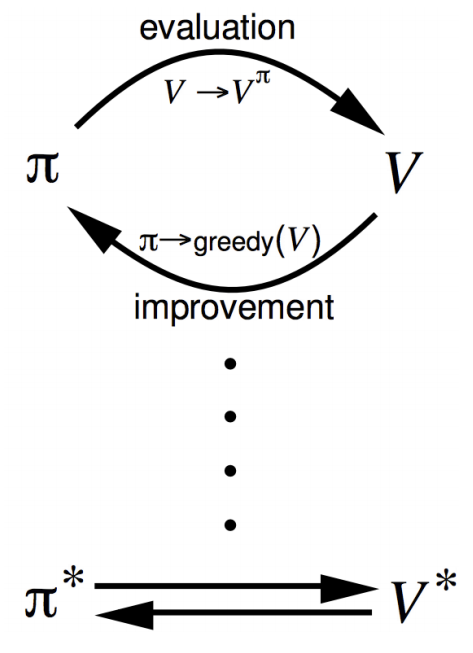
\includegraphics[width=0.3\textwidth]{Images/2_0_policy_iteration.png}
	\caption[Policy iteration algorithm]{Policy iteration algorithm \cite{sutton1998introduction}.}
	\label{fig:policy_iteration}
\end{figure}
  


